\documentclass[12pt]{book}
\usepackage{graphicx}
\usepackage{mathtools}
\usepackage{xcolor}
\usepackage{enumitem}
\usepackage{multirow}
\usepackage{booktabs}
\parindent 0pt
\parskip 6pt
\begin{document}
\title{
piHPSDR User's Manual
}
\author{
Christoph van W\"ullen, DL1YCF
}
%
\maketitle
\tableofcontents
\chapter{Introduction}
piHPSDR is a program that can operate with software defined radios (SDRs). As a graphical user interface,
it uses the GTK-3 toolkit, while the actual signal processing is done by Warren Pratt's WDSP library. Thus,
piHPSDR organizes the transfer of digitized radio frequency (RF) data between the radio hardware and the WDSP library, the
transfer of audio data (either from a microphone or to a headphone), as well as the processing of user
input (either by mouse/touch-screen, keyboard, or external "knobs and buttons"),
 and the graphical display of the RF data. piHPSDR is intended
to run on different variants of Unix. It runs on all sorts of Linux systems, including a Raspberry Pi (hence
the name piHPSDR), but equally well on Linux desktop or laptop computers, and on Apple Macintosh (Mac OSX)
computers which have a Unix variant under the hood. The present author is not aware of piHPSDR running
under the Windows operating system, although with environments such as MinGW, this should be possible.

Although piHPSDR can be operated entirely by using mouse and keyboard as input devices, many users prefer to
have physical push-buttons and/or knobs or dials. To this end, piHPSDR can control push-buttons and rotary
encoders connected to the GPIO (general purpose input/output)
lines of a Raspberry Pi. At least two generations of such controllers have
been put on the market by Apache labs, and I know of several projects where home-brewn controllers have
successfully been made. As an alternative, MIDI devices can be used for user interaction. For desktop/laptop
computers that do not have GPIO lines, MIDI offers an easy-to-use possibility of having push-bottons and
dials that control piHPSDR. Apart from homebrew projects in which a micro-controller such as an Arduino Micro
controls the actual buttons/knobs and acts as a MIDI device to the computer to which it is connected via USB,
there are low-cost so-called "DJ controllers" (DJ stands for disk jockey) from various brands which have
successfully been used with piHPSDR. A third possibility to control piHPSDR is via a serial interface
through CAT (computer aided transceiver) commands. The CAT model used by piHPSDR is based on the Kenwood
TS-2000 command set with lots of PowerSDR extensions.

Using a touch-screen instead of a mouse offers the possiblity to put the actual radio hardware together
with a Raspberry Pi running piHPSDR and an assortment of buttons/knobs into a single enclosure. This way,
one can build an SDR radio which can be operated like a conventional analog one.

The piHPSDR program has been written by John Melton G0ORX/N6LYT. It is free software that is licensed under
the GNU (free software foundation) general public license. Many other radio amateurs have contributed to
the code. A lot of extensions and improvements have been added by myself, therefore this document refers
to the version of piHPSDR that can be found on my github account \texttt{https://github.com/dl1ycf/pihpsdr}.

Because piHPSDR can be used on many different types of computers, and because operating systems change
rather quickly over time, I generally do not recommend to have a ,,binary release'' with files that you
can just copy to your computer and then it runs. Instead, my personal recommendation is to build piHPSDR
and WDSP from the sources, only this procedure guarantees compatibility of the final program with your
operating system. A manual of how to compile piHPSDR from the sources is available separately,
see \texttt{https://github.com/dl1ycf/pihpsdr-compile-from-sources}, so this will not be covered in 
the present manual. This manual starts with the first invocation of a freshly compiled piHPSDR.

\chapter{Starting piHPSDR for the first time}
Let us assume you have an SDR (say, an ANAN-7000 or a HermesLite-II) powered up and connected to an antenna,
and you have piHPSDR installed on a computer (say, a Raspberry Pi or an Apple Macintosh), the first thing to
do is to establish a proper connection between the computer and the radio. Although advocated at many places,
I do highly recommend against a WiFi connection. WiFi routers often use ,,optimizations'' where they hold
back data packets for a given client for a while, to be able to send a collection of them in a burst. While
this certainly optimizes the through-put because it minimizes clear-channel arbritration events, such jitters
are desastrous in SDR operation. The safest way of connecting the radio and the computer is to have a
managed switch with a built-in DHCP server, and to connect both the computer and the radio with a suitable
cable to the switch. If the computer has both a RJ45 jack for an ethernet cable, and a WiFi interface, my
personal recommendation is to use WiFi to connect to the internet, and use a single ,,direct cable'' plugged
into the RJ45 jacks of the computer and of the radio. This is a little bit tricky since both the computer
and the radio have to be set to a fixed IP address (e.g. computer: 192.168.1.50, radio: 192.168.1.51) with
the same netmask. However, once this has been done, this is the safest connection with no perturbations from
elsewhere.

\newpage
If the piHPSDR program is started for the first time, it opens a window that looks like this

\begin{center}
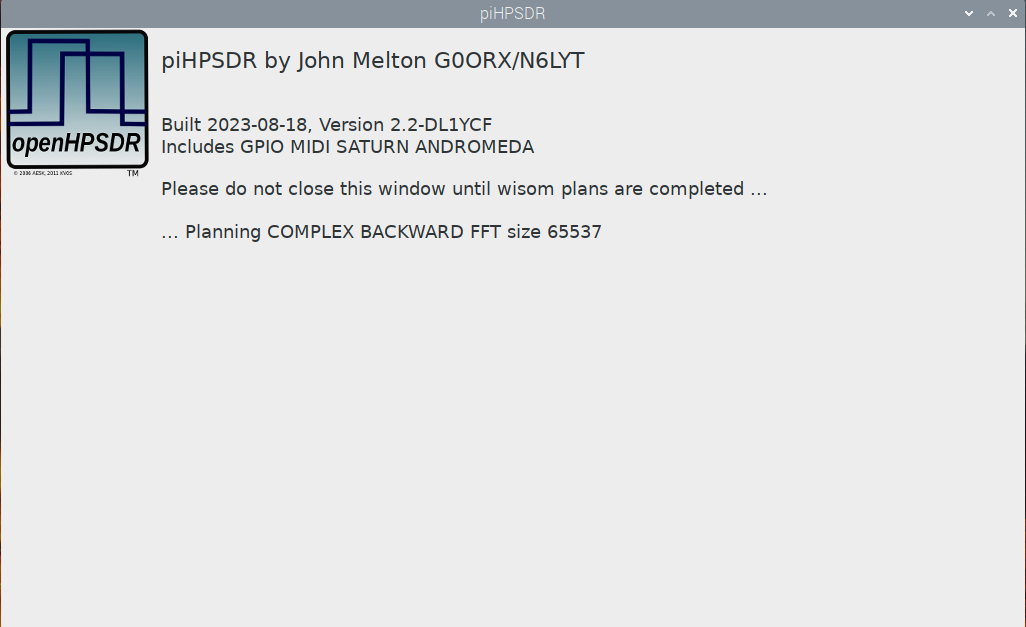
\includegraphics[width=12cm]{Planning.png}
\end{center}

besides stating a version number and when piHPSDR was built, a list of optional features (to be activated
at compile time) is stated, in this case, GPIO, MIDI, SATURN, and ANDROMEDA. These options indicate
that the program has GPIO support (this is only possible on Raspberry Pi or similar single board computers),
that is has support for MIDI devices, that it can run natively on the compute module of the latest
G2 (generation two) SDRs from Apache labs, and that is has support for Laurence Barker's ANDROMEDA controller.
What is important here that you have to wait. This only applies to the very first time you start piHPSDR.
On CPUs with a rather simple instruction set (like the ARM processor in the Raspberry Pi, or the Apple
Silicon processor in recent Macintosh computers), this "planning" step is quite fast, on CPUs with very
complex instruction sets like the Intel x86 processors, this step can last up to 15 minutes. When the
"wisdom plans" are completed, piHPSDR tries to detect a radio on the network. If everything went well with
the network connection, you then see a screen with a ,,discovery menu''

\begin{center}
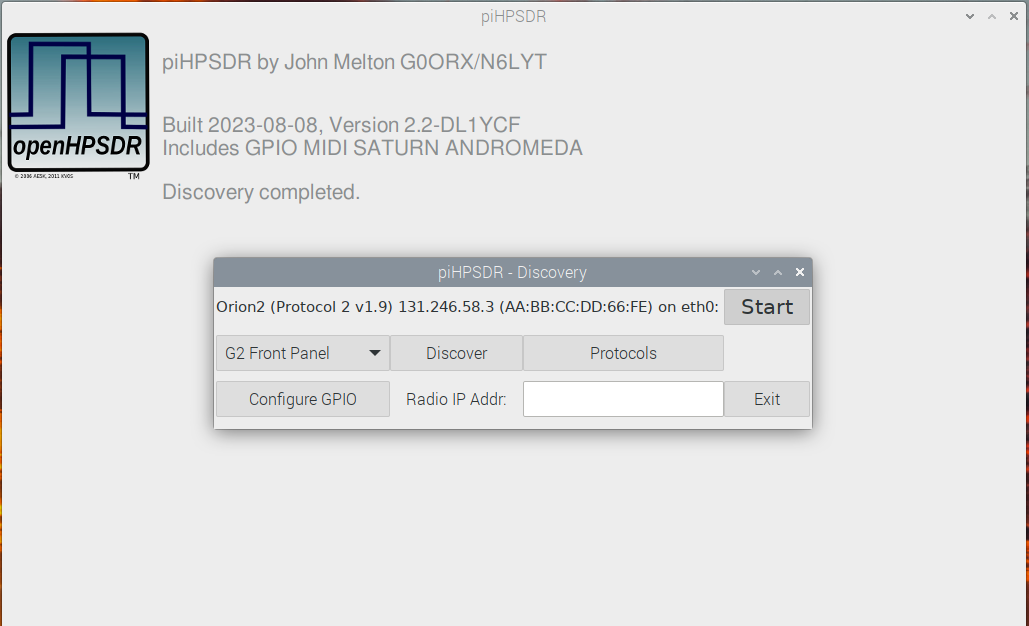
\includegraphics[width=12cm]{Start.png}
\end{center}

At this point, you can start the radio by clicking the \texttt{Start} button, but let us first explain the
purpose of the other buttons! Easiest to explain is the \texttt{Exit} button, this will simply terminate
the program. Most likely, you may want to go into the \texttt{Protocols} menu sooner or later.
 By default, piHPSDR tries to
discover the presence of a radio using all protocols known to piHPSDR. However, if you know that your radio, for
example, uses Protocol 2, then trying to discover a Protocol-1 radio is just a waste of time. So if you
know which types of radio you want to connect to, check these protocols. The available protocols are
\begin{itemize}[font=\texttt, left=80pt]
\item[Protocol 1]{This is the "original" HPSDR protocol.}
\item[Protocol 2]{This is the "new" HPSDR protocol.}
\item[Saturn XDMA]{This is used to talk to a Saturn FPGA through the internal XDMA interface. Only available
if piHPSDR is compiled with the \texttt{SATURN}  option.}
\item[USB OZY]{This is used to talk to a radio using the legacy USB OZY interface. Only available if piHPSDR
is compiled with the \texttt{USBOZY} option.}
\item[SoapySDR]{This is used to talk to a radio through the SoapySDR library, for example to an AdalmPLUTO. 
Only available if piHPSDR is compiled with the \texttt{SOAPYSDR} option.}
\item[STEMlab]{This is used to connect to RedPitaya based SDRs through the WEB interface. Only available if piHPSDR is
compiled with the \texttt{STEMLAB\_DISCOVERY} option. Starting the radio using this protocol is a two-step process:
first, the RedPitaya's WEB interface is located, and the \texttt{Start} button then starts the SDR app
on the RedPitaya. Then, piHPSDR tries to connect to this SDR app and upon success offers a new \texttt{Start} button
to start the radio. If the RedPitaya is exclusively used as a radio, it is recommended to auto-start the SDR app
when the RedPitaya is powered up. In this case, the STEMlab protocol is not used, because the SDR app can be started
through Protocol-2.}
\item[Autostart]{This is a very useful option. It indicates that if exactly one radio has been found, it is automatically
started. So in normal operation, when starting piHPSDR subsequently, and all settings are still valid, the radio is
started without user intervention. If this option is activated and one radio is present, you will not see this menu, so in order
to make further changes here, you have to disconnect the radio from the ethernet cable, start piHPSDR until you see this
menu, and reconnect the radio.}
\end{itemize}

Sometimes piHPSDR needs to know the IP address of the radio. This is, for example, the case for the \texttt{STEMlab} discovery
described above. In such a case the IP address in numerical form (xxx.xxx.xxx.xxx) can be entered in the box
with the label \texttt{Radio IP Addr:}. If a legal IP address is contained in this box, protocol-1 and protocol-2 discoveries
will also send, in addition to a broadcast discovery packet, such a packet to the IP address specified. This way one can
connect to radios which are not on the same subnet as the computer, in principle you can connect to any radio on the world
provided it is on the internet. However, the original HPSDR standard states that a broadcast packet must be used, so several
radios won't reply. On the other hand, there are some radios such as a RedPitaya or a HermesLite-II which allow being discovered
by such a routed packet. 

The \texttt{Discover} button re-starts the discovery process. This is useful if the radio has been powered up too late and
was not yet ready when piHPSDR was started. Simply press \texttt{Discover} to give another try.

The \texttt{Configure GPIO} button opens a menu that currently has no function, so it is not described here.

The combo-box (pop-down menu) to the left of the \texttt{Discover} button lets you choose which type of GPIO controller you
have attached to the computer. This menu is only available if piHPSDR has been compiled with the \texttt{GPIO} option, which
is not the case on desktop/laptop computers. The menu lets you choose between

\begin{itemize}[font=\texttt, left=80pt]
\item[No Controller]{Choose this if no GPIO controller is wired to your Raspberry Pi.}
\item[Contoller1]{Choose this if you have a "version 1" piHPSDR controller.}
\item[Controller2 V1]{This option is valid for some early prototypes of the "version 2" controller.}
\item[Controller2 V2]{Choose this if you have a "version 2" piHPSDR controller.}
\item[G2 Front Panel]{Choose this if you have an ANAN G2 radio with a built-in controller.}
\end{itemize}

\textbf{Attention.} Be sure to choose a controller only if such a controller is actually connected to your Raspberry Pi. If
you choose, for example, a controller which uses an I2C expander for the switches, but no I2C interface is present on
your Raspberry Pi, the program my hang when trying to open the I2C connection.

All settings (protocols, controller, IP address) made in this menu are stored in the global (radio-indepentend) settings
and are restored when piHPSDR is started the next time. 

If all went well, a radio could be discovered and you hit the \texttt{Start} button, you should see the following

\begin{center}
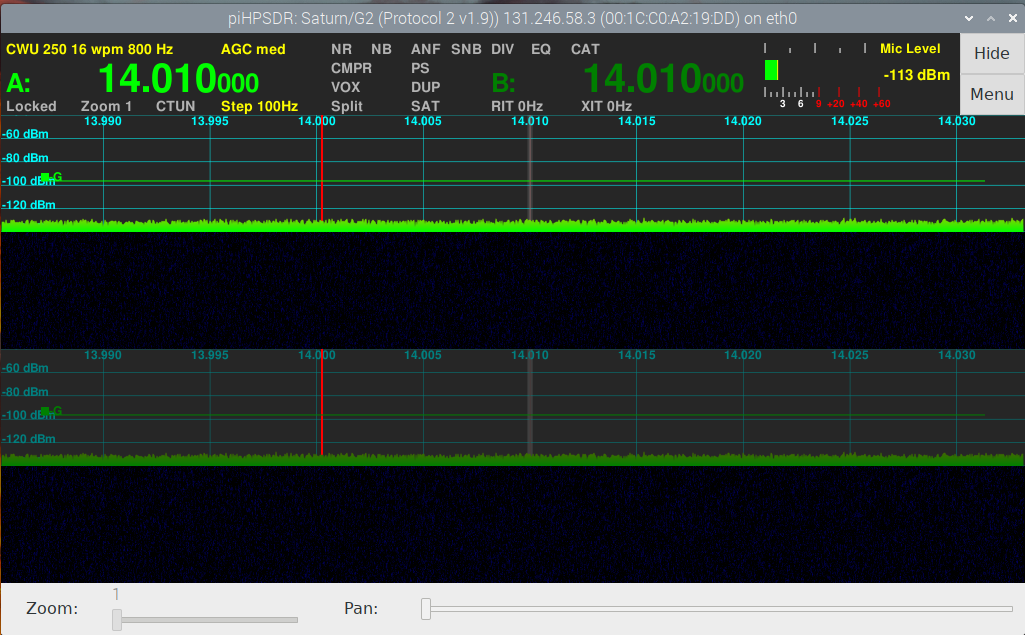
\includegraphics[width=12cm]{FirstDisplay.png}
\end{center}

The bottom of the window looks different (more controls) if you have chosen \texttt{No Controller} in the preceeding menu.
You see two receiver panels stacked vertically, both of them having a spectrum display and a waterfall area. At the top,
just below the window title, you have the VFO bar which contains information on the frequencies of the two VFOs A and B,
as well as lots of further information, to be explained later. At the top right, there are two buttons \texttt{Hide}
and \texttt{Menu} which will be explained in the next chapter. To the left of these two buttons, there is the meter
bar which by default is a digital S-meter. At this point, you have started piHPSDR successfully for the first time.

\chapter{Main window layout}

\begin{center}
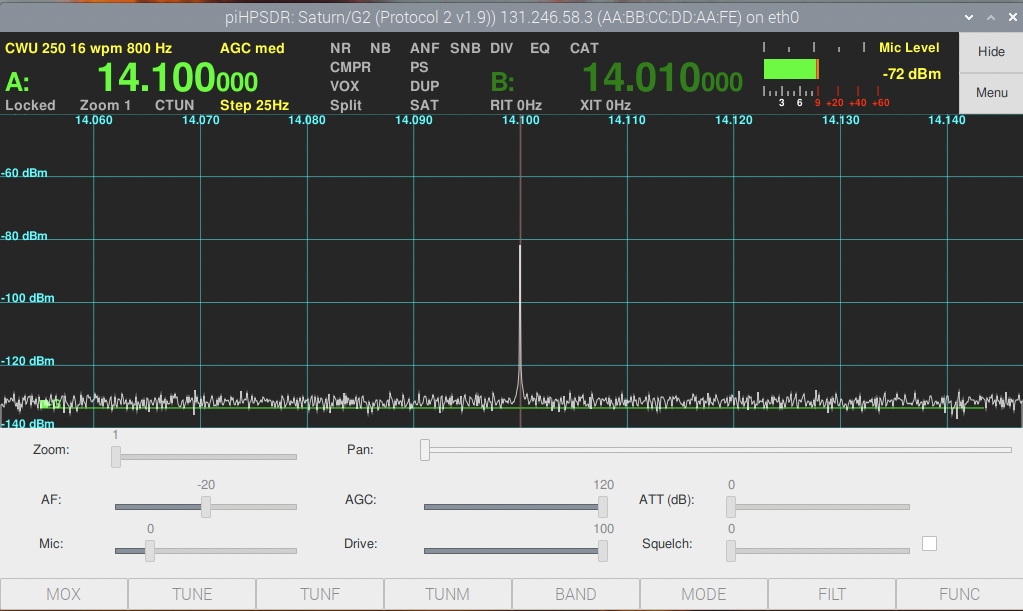
\includegraphics[width=12cm]{SingleReceiver.png}
\end{center}


\begin{center}
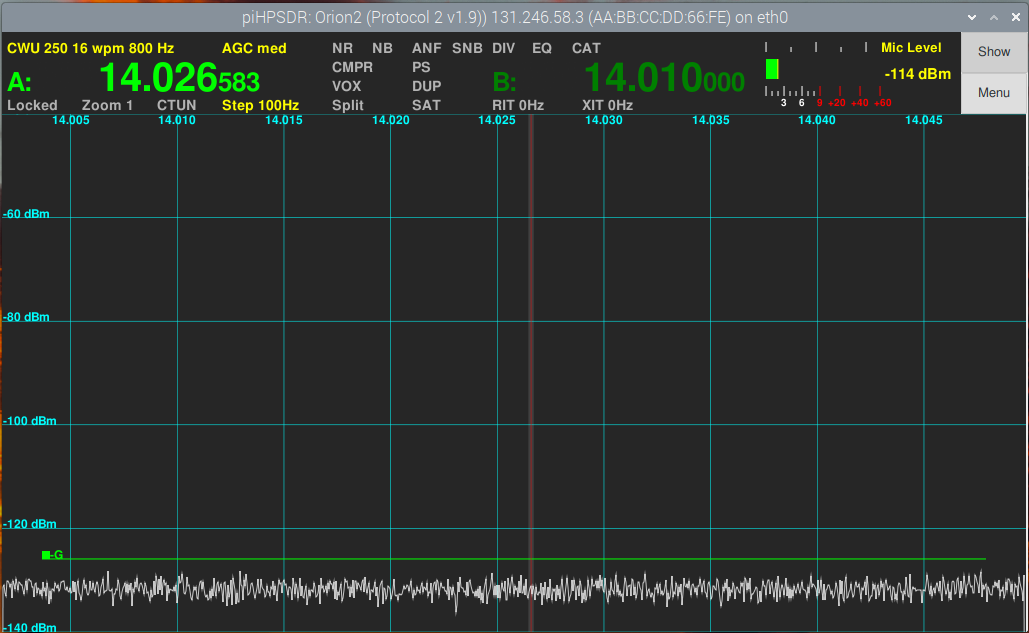
\includegraphics[width=12cm]{Hidden.png}
\end{center}

\section{Window areas}

\section{VFO bar and status  indicators}

\section{Meter section}


\chapter{The Main Menu: introduction}

\begin{center}
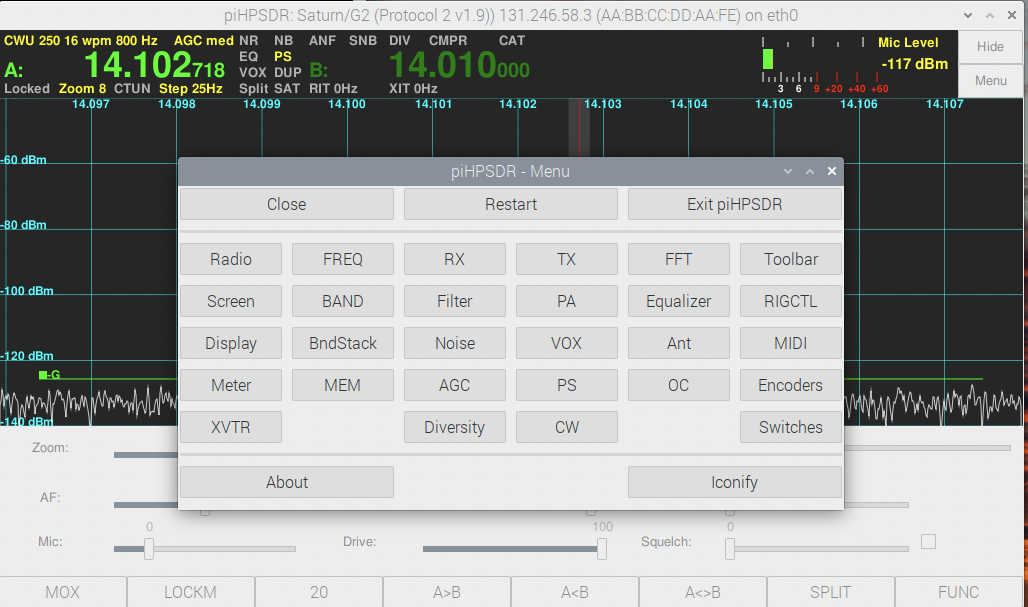
\includegraphics[width=12cm]{MainMenu.png}
\end{center}

\section{The \texttt{Exit} Menu}
\begin{center}
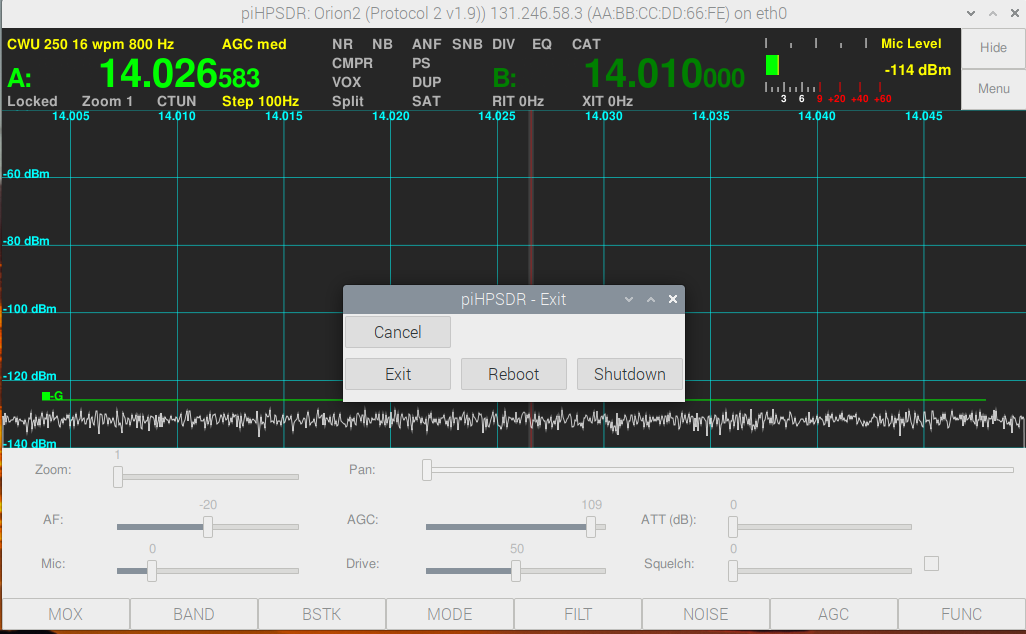
\includegraphics[width=12cm]{ExitMenu.png}
\end{center}

\section{The \texttt{About} Menu}
\begin{center}
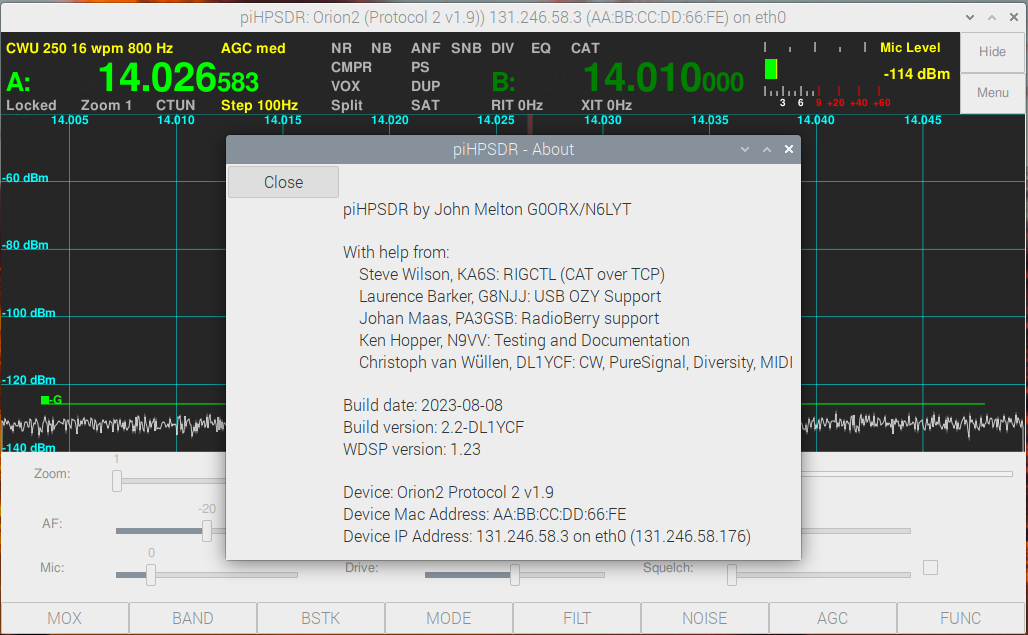
\includegraphics[width=12cm]{AboutMenu.png}
\end{center}

\chapter{The Main Menu: Radio-related menus}

\section{The \texttt{Radio} Menu}
\begin{center}
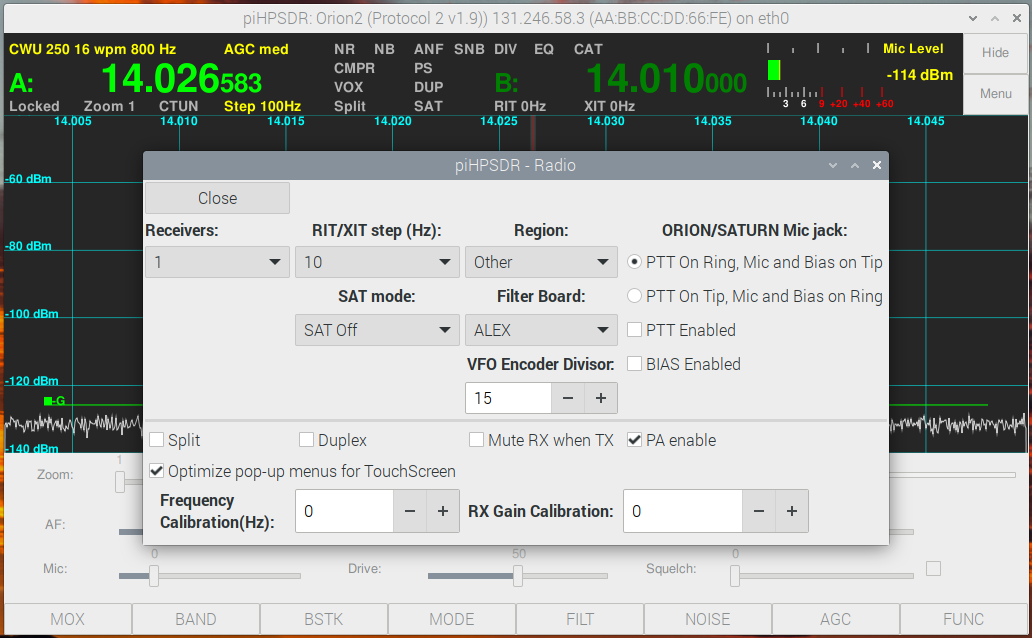
\includegraphics[width=12cm]{RadioMenu.png}
\end{center}

\section{The \texttt{Screen} Menu}
\begin{center}
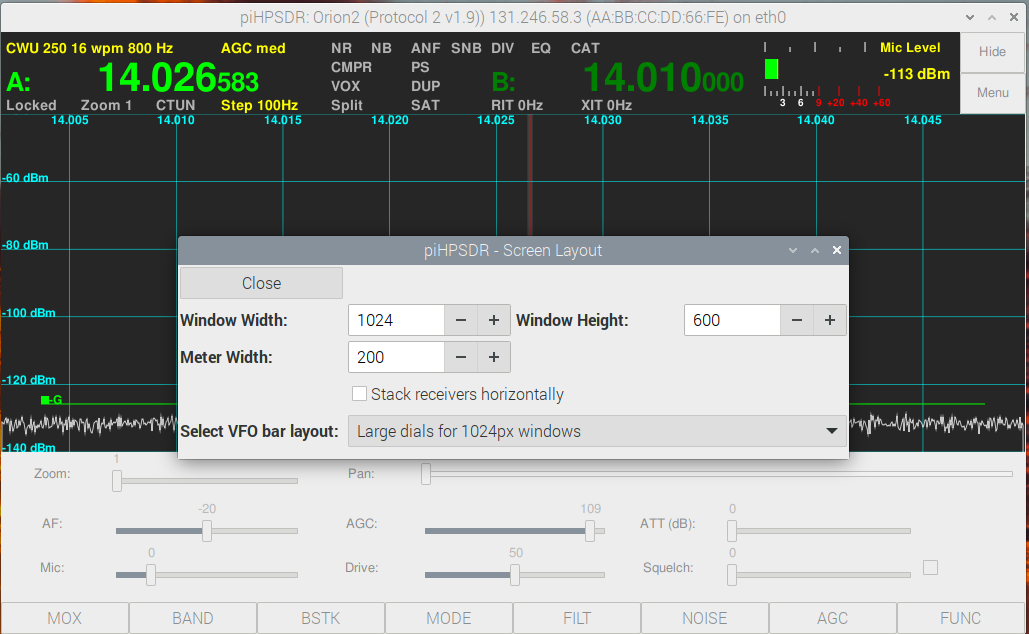
\includegraphics[width=12cm]{ScreenMenu.png}
\end{center}

\section{The \texttt{Display} Menu}
\begin{center}
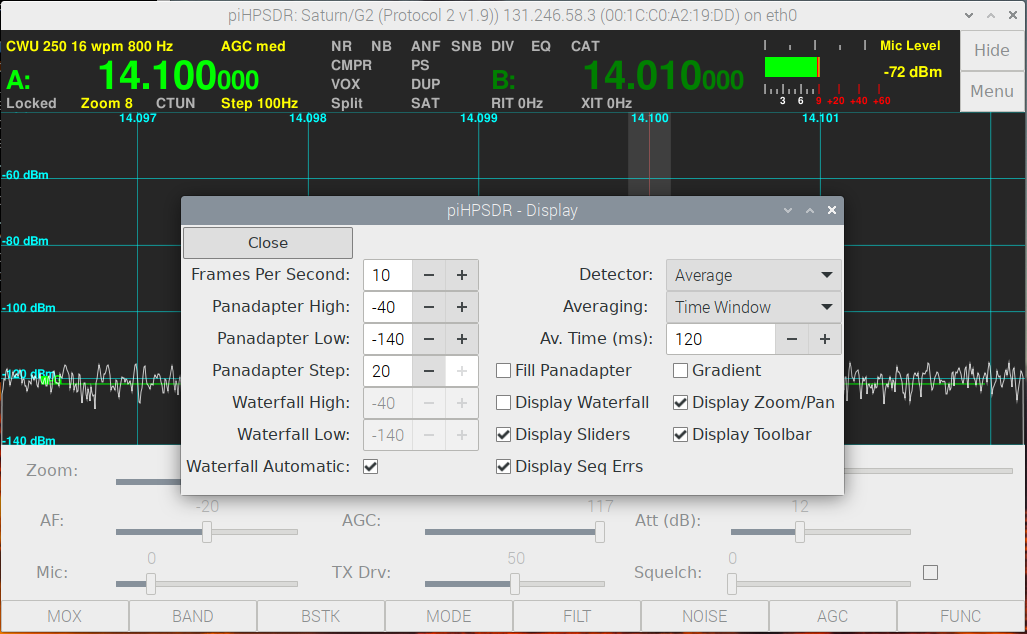
\includegraphics[width=12cm]{DisplayMenu.png}
\end{center}

\section{The \texttt{Meter} menu}
\begin{center}
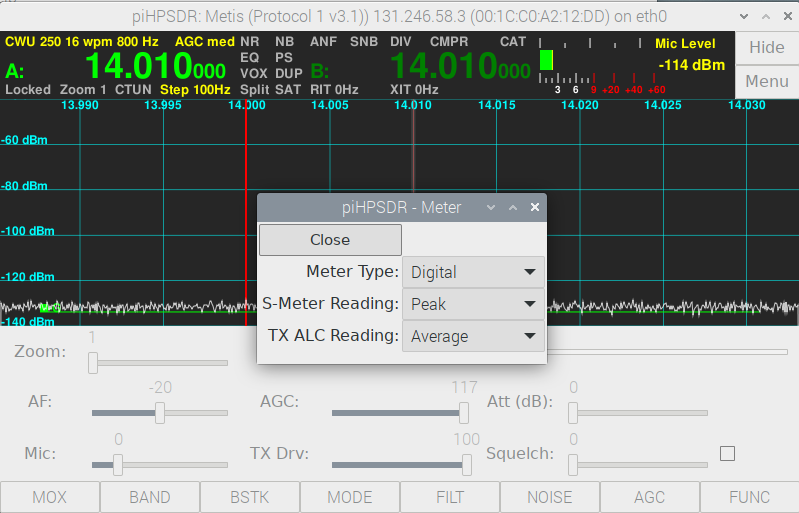
\includegraphics[width=12cm]{MeterMenu.png}
\end{center}

\section{The \texttt{XVTR} (Transverter) Menu}
\begin{center}
\includegraphics[width=12cm]{XVTRMenu.png}
\end{center}

\chapter{The Main Menu: VFO-related menus}

\section{The \texttt{FREQ} (VFO) menu}
\begin{center}
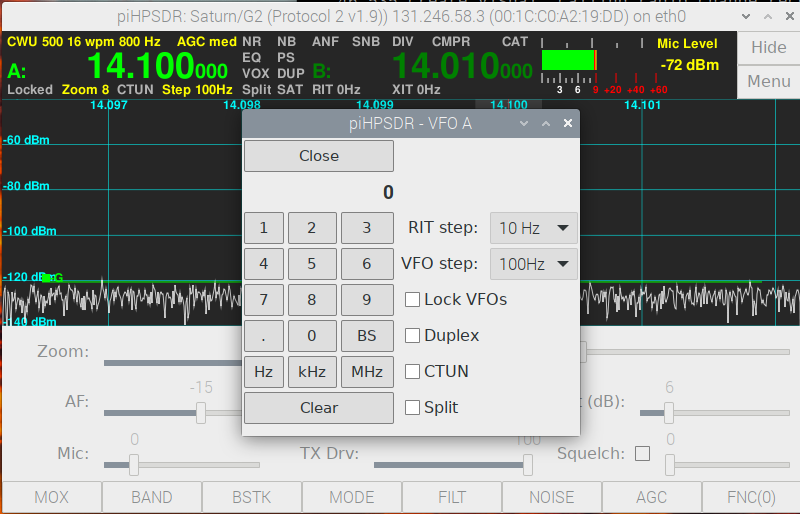
\includegraphics[width=12cm]{VFOmenu.png}
\end{center}

\section{The \texttt{Band} menu}
\begin{center}
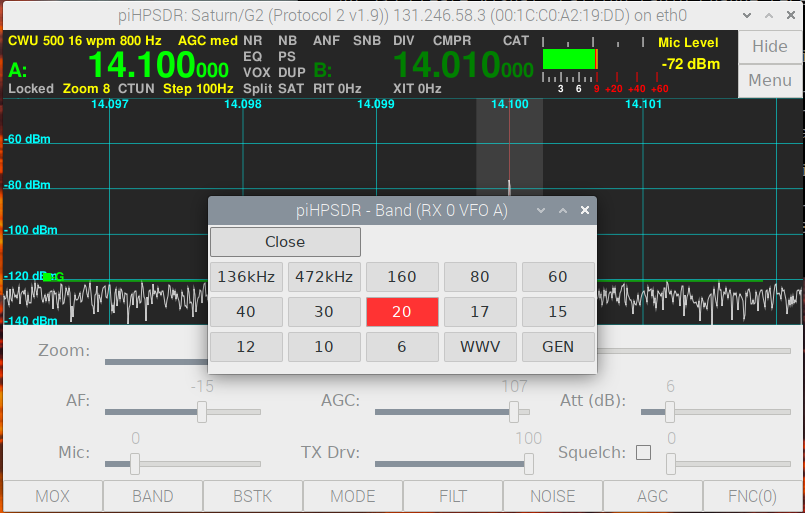
\includegraphics[width=12cm]{BandMenu.png}
\end{center}

\section{The  \texttt{BStack} (Bandstack) menu}
\begin{center}
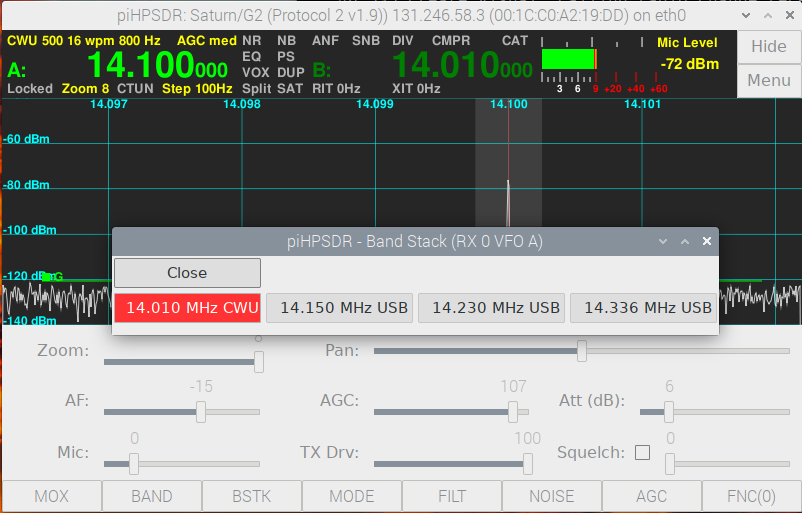
\includegraphics[width=12cm]{BandstackMenu.png}
\end{center}
 
\section{The \texttt{Mode} menu}
\begin{center}
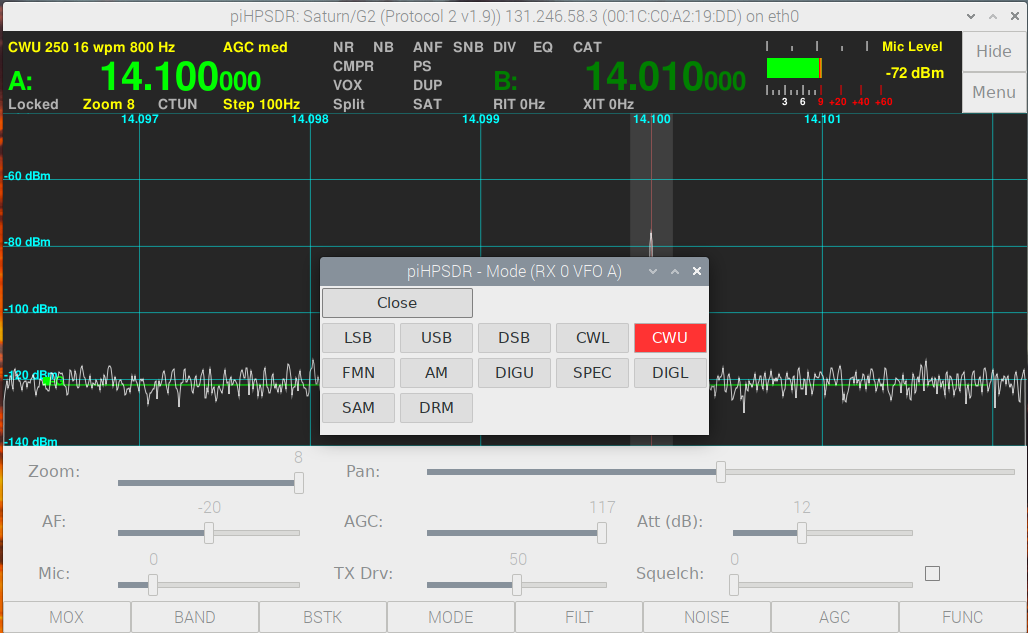
\includegraphics[width=12cm]{ModeMenu.png}
\end{center}

\section{The \texttt{MEM} (Memory) menu}

 
\chapter{The Main Menu: RX-related menus}

\section{The \texttt{RX} Menu}
\begin{center}
\includegraphics[width=12cm]{RXMenu.png}
\end{center}

\section{The \texttt{Filter} menu}
\begin{center}
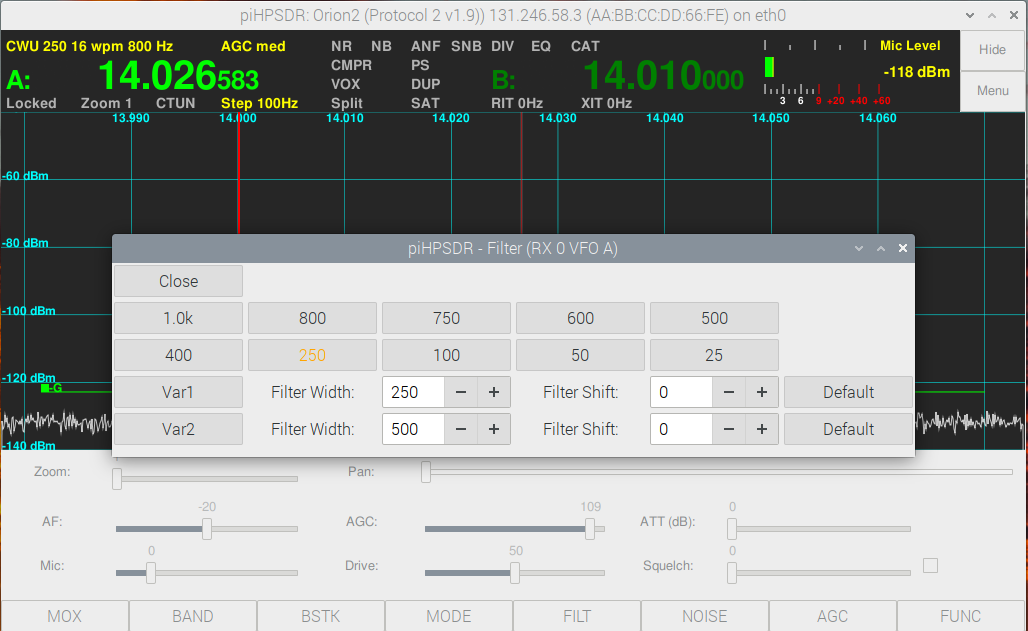
\includegraphics[width=12cm]{FilterMenu.png}
\end{center}

\section{The \texttt{Noise} Menu}
\begin{center}
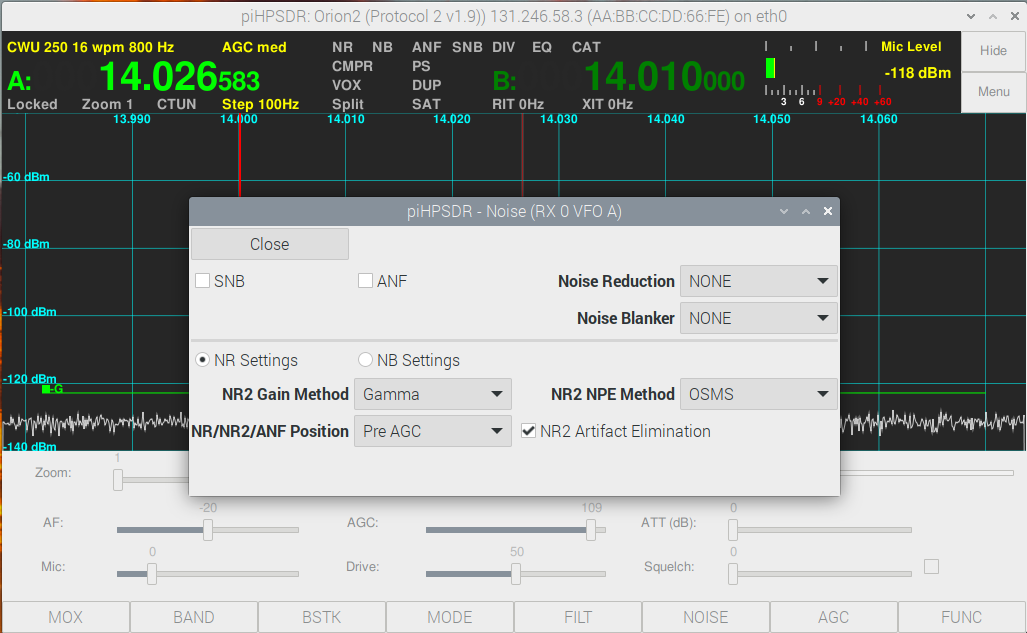
\includegraphics[width=12cm]{NoiseMenu.png}
\end{center}

\section{The \texttt{AGC} Menu}
\begin{center}
\includegraphics[width=12cm]{AGCMenu.png}
\end{center}

\section{The \texttt{Diversity} Menu}
\begin{center}
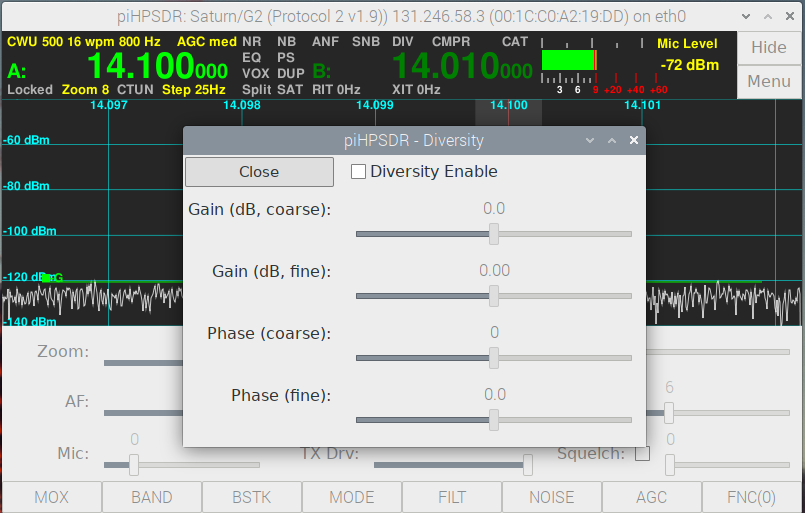
\includegraphics[width=12cm]{DiversityMenu.png}
\end{center}

\chapter{The Main Menu: TX-related menus}

\section{The \texttt{TX} Menu}
\begin{center}
\includegraphics[width=12cm]{TXMenu.png}
\end{center}

\section{The \texttt{PA} Menu}
\begin{center}
\includegraphics[width=12cm]{PAMenuCalibrate.png}
\end{center}

\begin{center}
\includegraphics[width=12cm]{PAMenuWatt.png}
\end{center}

\section{The \texttt{VOX} Menu}
\begin{center}
\includegraphics[width=12cm]{VOXMenu.png}
\end{center}

\section{The \texttt{PS} (PureSignal) Menu}
\begin{center}
\includegraphics[width=12cm]{PSMenu.png}
\end{center}

\section{The \texttt{CW} Menu}
\begin{center}
\includegraphics[width=12cm]{CWMenu.png}
\end{center}

\chapter{The Main Menu: menus for RX and TX}

\section{The \texttt{FFT} (Signal Processing) Menu}
\begin{center}
\includegraphics[width=12cm]{FFTMenu.png}
\end{center}

\section{The \texttt{Equalizer} Menu}
\begin{center}
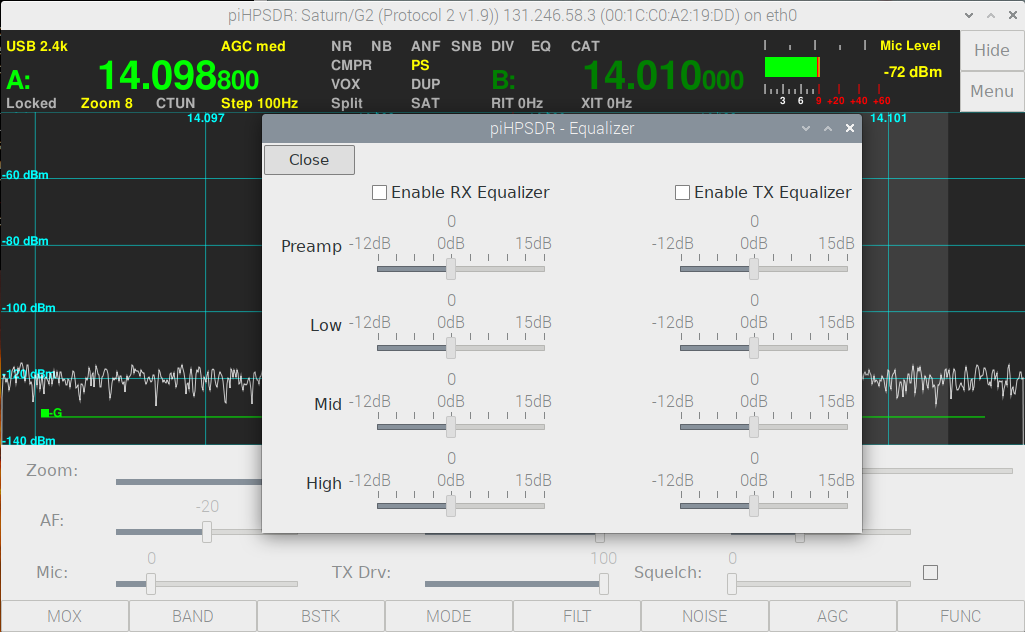
\includegraphics[width=12cm]{EqualizerMenu.png}
\end{center}

\section{The \texttt{Ant} (Antenna) Menu}
\begin{center}
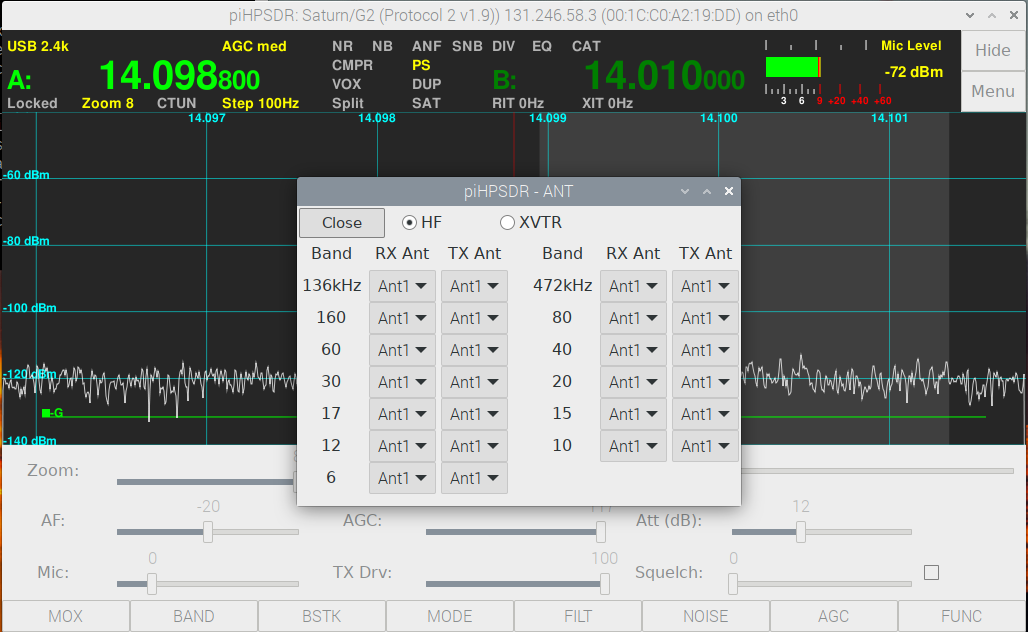
\includegraphics[width=12cm]{AntMenu.png}
\end{center}
 
\section{The \texttt{OC} (OpenCollector) Menu}
\begin{center}
\includegraphics[width=12cm]{OCMenu.png}
\end{center}

\chapter{The Main Menu: controlling piHPSDR}

In this chapter, the customization of the toolbar (at the bottom of the piHPSDR window),
as well as how to configure GPIO and MIDI controllers, is described. Furthermore, in this
chapter we discuss the RIGCTL menu which allows controlling piHPSDR by some external program
such as a logbook or contest program, via standardized CAT commands that can be sent to
piHPSDR either over a serial line or via TCP.

\textbf{Note for Controller1 owners:} The eight switches (push-buttons) of the controller,
that a positioned below the screen, are bound to the eight toolbar buttons on the screen.
Therefore, there is no "Switches" menu for this controller, and the switches are implicitly
configured via the Toolbar menu.

\section{The \texttt{Toolbar} Menu}
We start with the "Toolbar" menu, that can be found at the top of the rightmost
column in the main menu. The toolbar consists of eight buttons that can be assigned
to a set of eight functions. There are six such sets, and pressing the FUNC button
cycles through these six sets. If you click the Toolbar button, a menu pops up and
you see the following:

\begin{center}
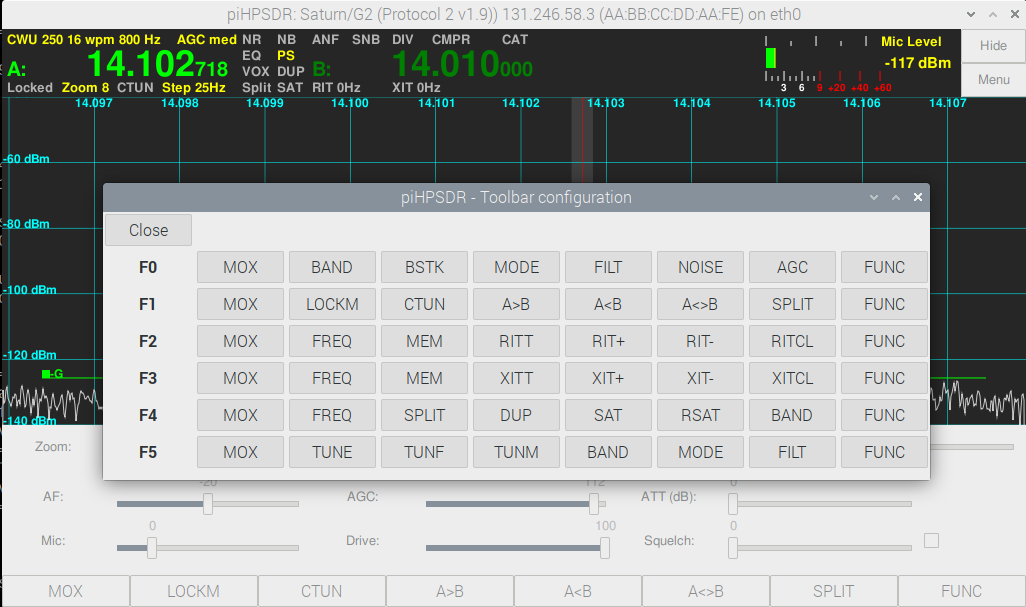
\includegraphics[width=12cm]{ToolbarMenu1.png}
\end{center}

The six lines denoted \texttt{F0} through \texttt{F5} indicate the six different sets. If you
look closely, you will discover that the set \texttt{F1} is the one that is currently active,
since the labels in this line exactly match the labels in the toolbar. In this menu, the
possible actions (that can be bound to a button) are written with the short text (see Chapter \ref{ch:actions}),
since this is the text that is printed on the toolbar buttons. If one now clicks (just an example)
the \texttt{CTUN} button in the line \texttt{F1}, an ,,action dialog'' pops up that looks as follows:

\begin{center}
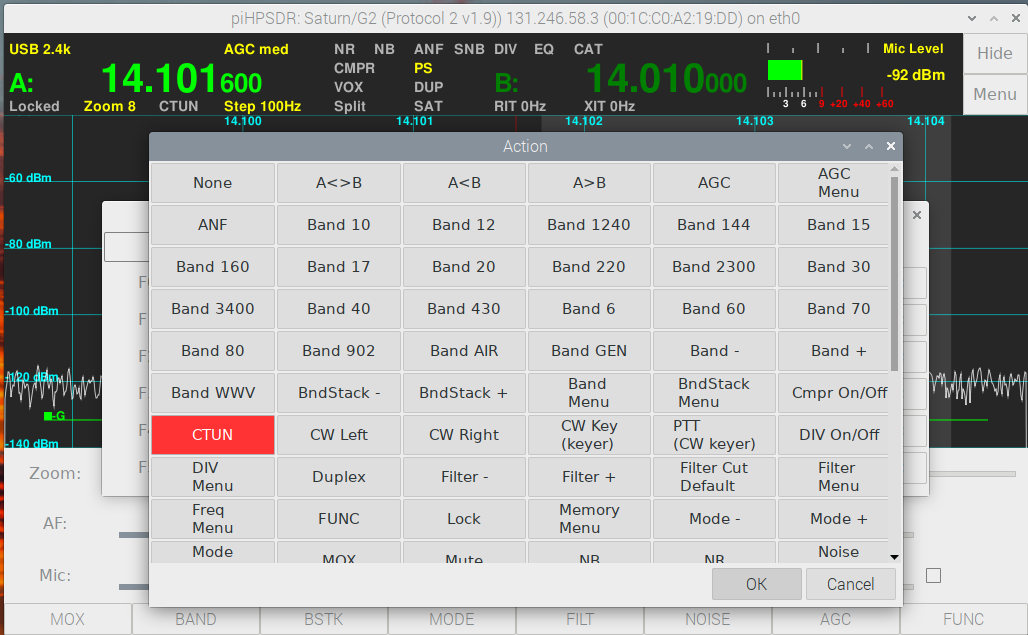
\includegraphics[width=12cm]{ToolbarMenu2.png}
\end{center}

The current action selected (\texttt{CTUN}) is high-lighted. Lists of possible actions can be rather long,
so it might be necessary that you have to scroll up or down in such an action dialog until you have
found what you were looking for. Now (again just an example) the button \texttt{Band 20} has been clicked
in the action dialog, such that it gets high-lighted:

\begin{center}
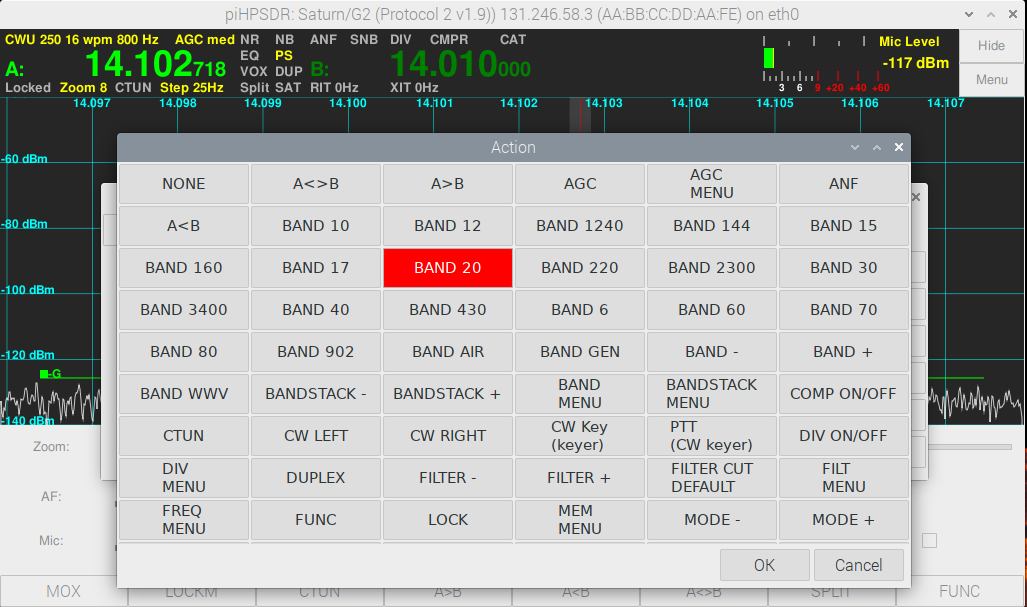
\includegraphics[width=12cm]{ToolbarMenu3.png}
\end{center}

If one now closes the action dialog by clicking the \texttt{OK} button, the third button in the \texttt{F1}
line of the toolbar menu has changed, it now gives the short text (\texttt{20}) of the action, which will
switch the active receiver to the 20m band (see the explanation of all the actions in chapter \ref{ch:actions}).

\begin{center}
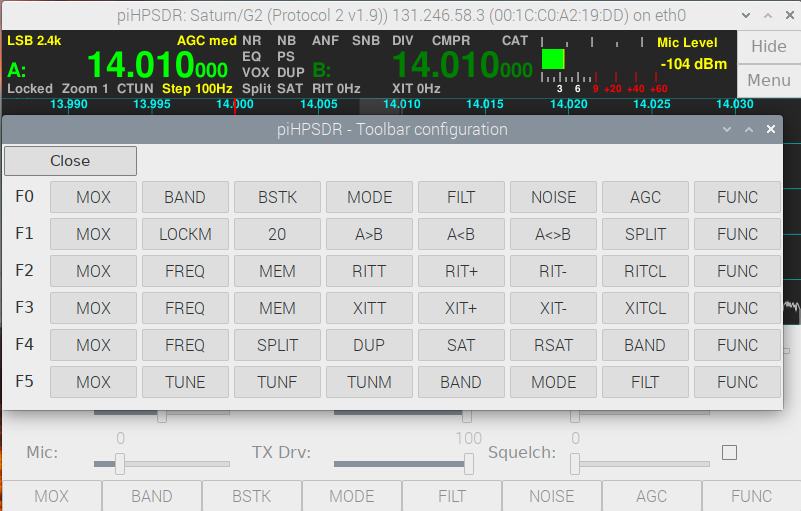
\includegraphics[width=12cm]{ToolbarMenu4.png}
\end{center}
You also see that the toolbar has changed, now reading \texttt{20} on the third button from the left. Note that
you can likewise change the functions of the toolbar sets that are currently not active, for example, we can
change the behaviour of a toolbar button in set \texttt{F5}, no matter whether this set is currently active
or not. Note futher that nothing happens if you press the \texttt{FUNC} buttons in the toolbar menu, since the
rightmost button is hard-wired to that function. This is so because if in one set, you do not have the 
\texttt{FUNC} functions at hand, you are trapped and can no longer cycle through the sets.

Assigning actions to buttons, as done here in the ,,action dialog'' also works, exactly as described here,
in the MIDI, the Encoders, and the Switches menus.


\section{The \texttt{RIGCTL} (CAT control) Menu}
\begin{center}
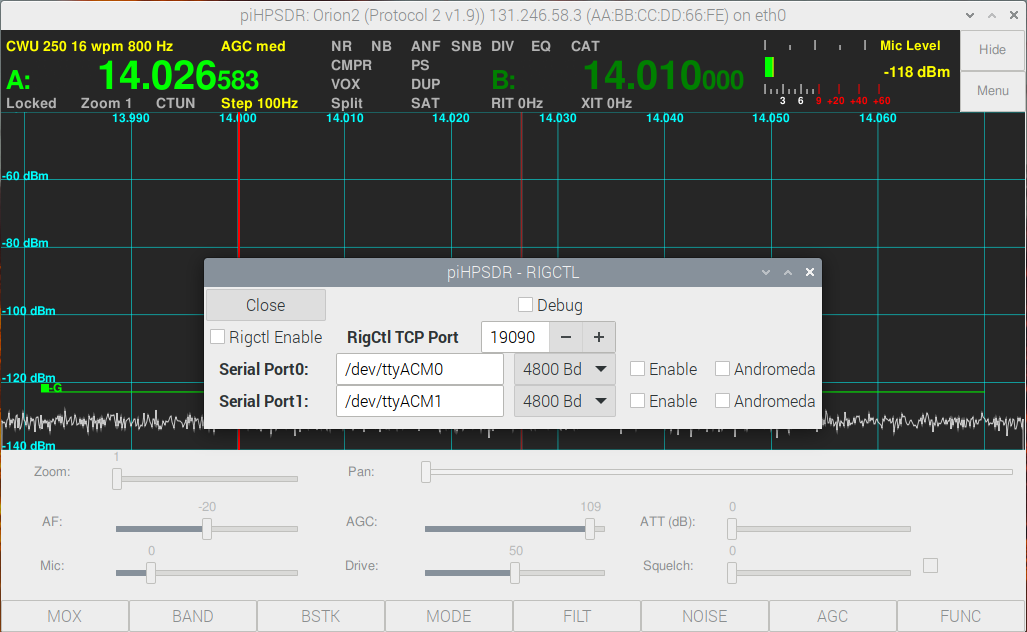
\includegraphics[width=12cm]{RigCtlMenu.png}
\end{center}

\section{The \texttt{MIDI} Menu}
\begin{center}
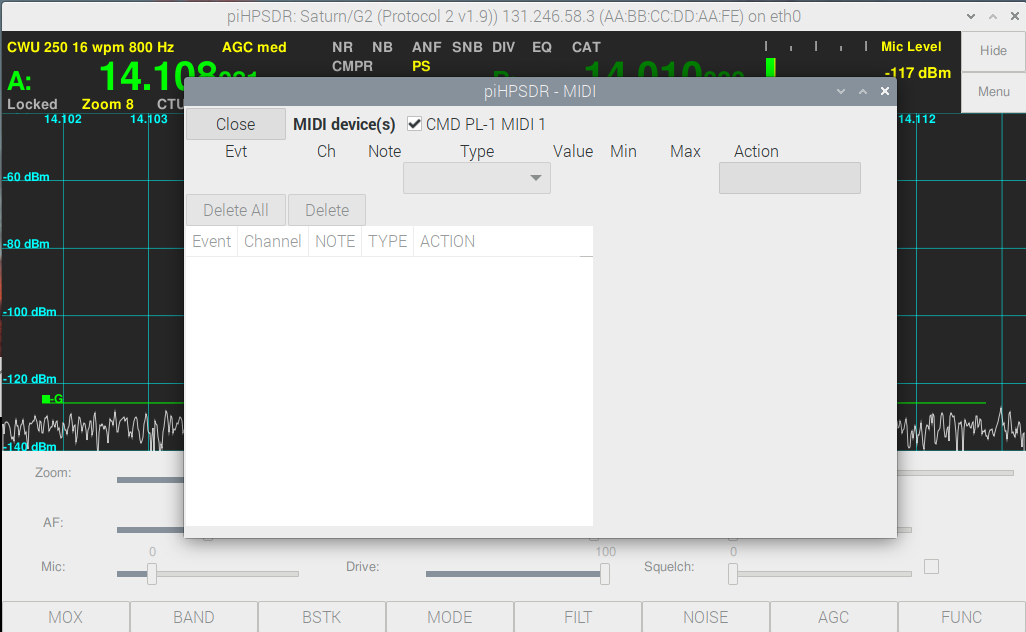
\includegraphics[width=12cm]{MIDImenu1.png}
\end{center}

\begin{center}
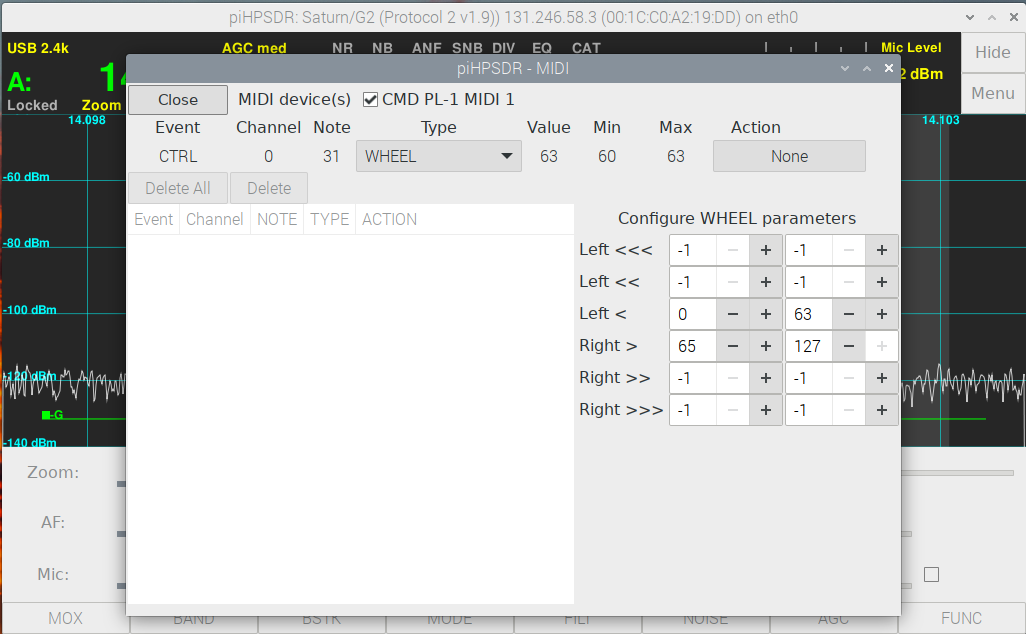
\includegraphics[width=12cm]{MIDImenu2.png}
\end{center}

\begin{center}
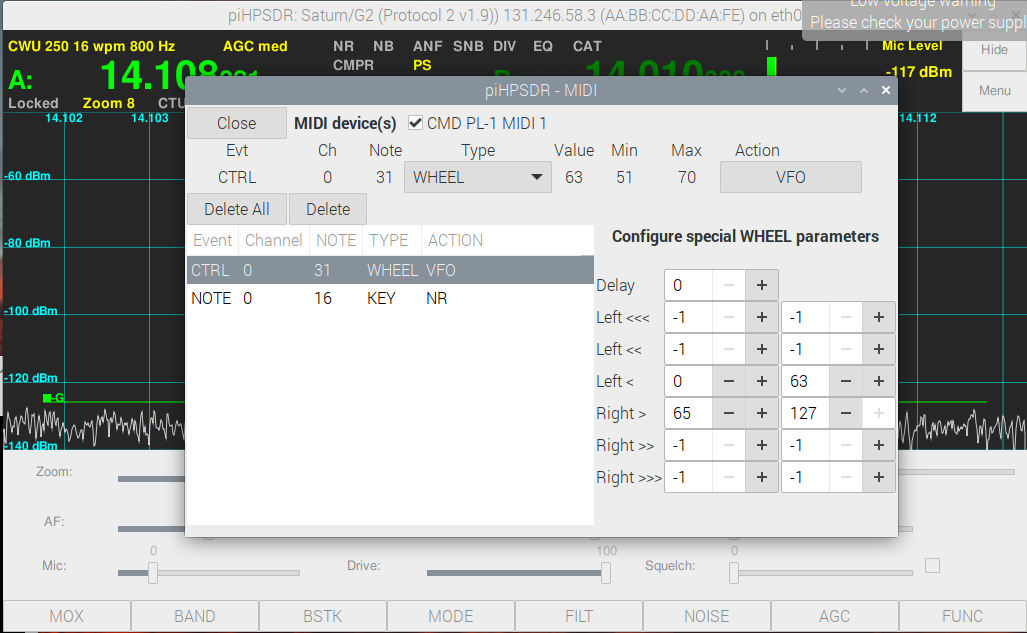
\includegraphics[width=12cm]{MIDImenu3.png}
\end{center}
 
\section{The \texttt{Encoders} Menu}
\begin{center}
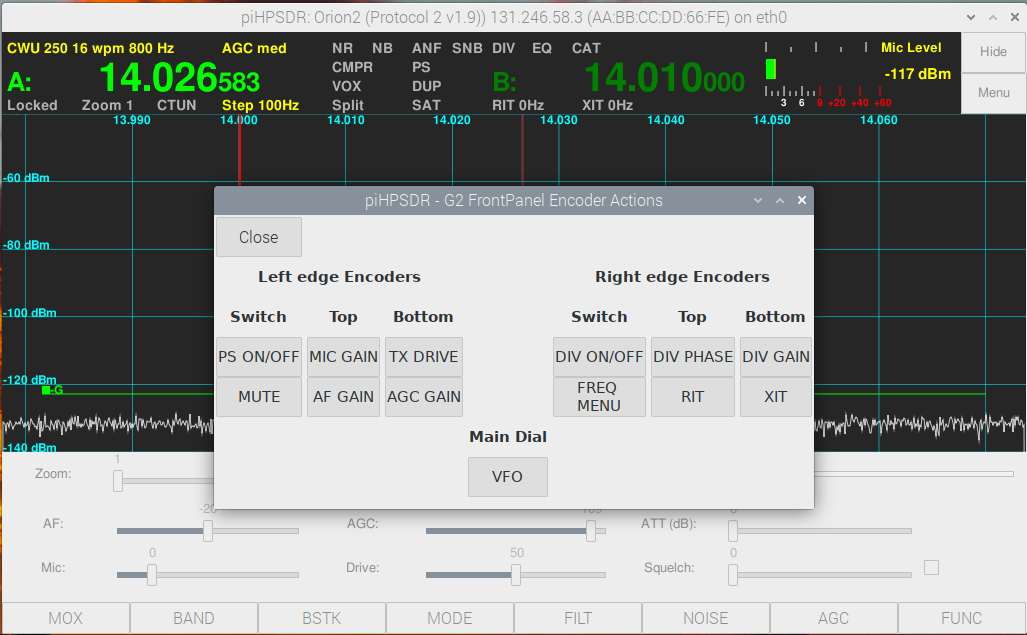
\includegraphics[width=12cm]{EncodersMenu.png}
\end{center}

\section{The \texttt{Switches} Menu}
\begin{center}
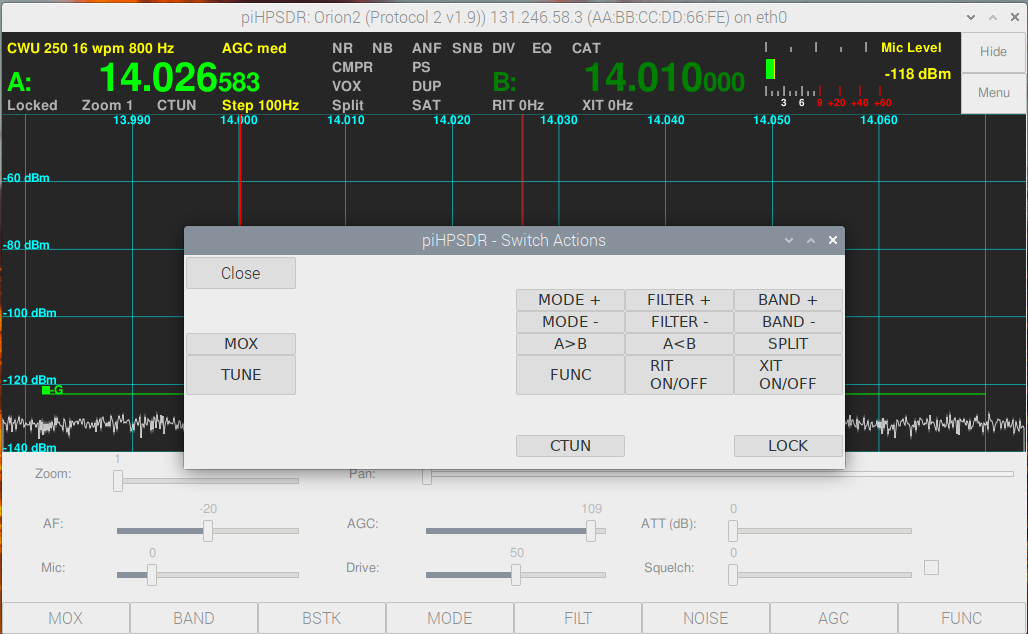
\includegraphics[width=12cm]{SwitchesMenu.png}
\end{center}

\chapter{List of piHPSDR ,,Actions''}
\label{ch:actions}

In this chapter, we give a list of ,,actions'' implemented in the piHPSDR program. These actions can be assigned to
toolbar buttons on the screen, or pushbuttons/encoders of a GPIO-connected or MIDI controller. Not all actions can
be assigned to all control elements. Changing the AF volume, for example, can only be assigned to a knob which
you can turn, while switching RIT on/off can only be assigned to a button that you can push. For each action
in the following table, there is a long and a short string assigned. The long string will be used when there is
enough space, while the short string is used for small buttons and to store actions in preference files (therefore
the short strings never contain a blank character or a line break). Then, for each action we give the type of control
element allowed for this action as a combination of the letters B, P, E, which stand for

\begin{itemize}[font=\texttt, left=0pt]
\item[B] {"Button": A button in the toolbar, or a push-button or switch on a GPIO or MIDI connected console}
\item[P] {"Potentiometer": A potentiometer or a slider on a MIDI connected console}
\item[E] {"Encoder": A rotary encoder on a GPIO or MIDI connected console}
\end{itemize}

The main difference between a "potentiometer" and an "encoder" is, that the former has a min and max position, while
an encoder can be turned in either direction without stopping. This means that a potentiometer
reports a value between min and max, while an encoder reports an increment,
that is, whether it has been turned clock wise or counter clock wise.
The existing GPIO consoles do not have potentiometers (most likely because of the lack of analog inputs), but
many MIDI consoles do have, and Arduino-based MIDI controllers might have it because there analog inputs
to read out potentiometers are available.

To give an example, controlling the TX drive can be down both with a slider and with an encoder. While for
a slider/potentiometer, the values from min to max are simple mapped to the TX drive values from 0 to 100,
the signals from an encoder will just increase or decrease the value until one of a limits has been reached.

In the following, the actions are alphabetically sorted by their long name, with the "empty" action listed
first.

\renewcommand{\belowrulesep}{0pt}
\renewcommand{\aboverulesep}{0pt}
\def\action#1#2#3#4{
\begin{center}
\begin{tabular}{|p{5cm}|p{5cm}|p{1cm}|}
\toprule
$\phantom{\Big|}$\texttt{\large #1} & \texttt{\large #2} & \texttt{\large #3} \\\cline{1-3}
\multicolumn{3}{|p{\textwidth}|}{#4} \\
\bottomrule
\end{tabular}
\end{center}
}


\action{NONE}{NONE}{BPE}{This is an action which does nothing. It can be assigned to buttons or enco\-ders that
are often accidentally operated. Some MIDI consoles, for example, report a button press event if the VFO
knob is touched, and this we want to ignore.}

\action{A<>B}{A<>B}{B}{Swap VFOs A and B. This will not only swap the frequencies, but also all other settings
associated with that VFO, such as mode, filter, CTUN, and RIT settings.}

\action{A<B}{A<B}{B}{Copy VFO B to VFO A.}

\action{A>B}{A>B}{B}{Copy VFO A to VFO B.}

\action{AF GAIN}{AFGAIN}{PE}{Change the AF gain (headphone volume) of the active receiver.}

\action{AF GAIN RX1}{AFGAIN1}{PE}{Change the AF gain (headphone volume) of the RX1 receiver.}

\action{AF GAIN RX2}{AFGAIN2}{PE}{Change the AF gain (headphone volume) of the RX2 receiver.}

\action{AGC MENU}{AGC}{B}{Opens the \texttt{AGC} menu.}

\action{ANF}{ANF}{B}{Toggels the state (on/off) of the automatic notch filter for the active receiver.}

\action{ATTEN}{ATTEN}{PE}{Changes the value (0-31 dB) of the step attenuator of the active receiver.
This funciton is only available for radios that have such an attenuator.}

\action{BAND 10}{10}{B}
{Change band of the active receiver to the 10m band. If already on that band, move to
the next bandstack entry. This action is a no-op if the frequency of the band falls outside the frequency range
of the radio.} 

\action{BAND 12}{12}{B}
{Change band of the active receiver to the 12m band. If already on that band, move to
the next bandstack entry. This action is a no-op if the frequency of the band falls outside the frequency range
of the radio.}

\action{BAND 1240}{1240}{B}
{Change band of the active receiver to the 1240 MHz (23 cm) band. If already on that band, move to
the next bandstack entry. This action is a no-op if the frequency of the band falls outside the frequency range
of the radio.}

\action{BAND 144}{144}{B}
{Change band of the active receiver to the 144 MHz (2m) band. If already on that band, move to
the next bandstack entry. This action is a no-op if the frequency of the band falls outside the frequency range
of the radio.}

\action{BAND 15}{15}{B}
{Change band of the active receiver to the 15m band. If already on that band, move to
the next bandstack entry. This action is a no-op if the frequency of the band falls outside the frequency range
of the radio.}

\action{BAND 160}{160}{B}
{Change band of the active receiver to the 160m band. If already on that band, move to
the next bandstack entry. This action is a no-op if the frequency of the band falls outside the frequency range
of the radio.}

\action{BAND 17}{17}{B}
{Change band of the active receiver to the 15m band. If already on that band, move to
the next bandstack entry. This action is a no-op if the frequency of the band falls outside the frequency range
of the radio.}

\action{BAND 20}{20}{B}
{Change band of the active receiver to the 15m band. If already on that band, move to
the next bandstack entry. This action is a no-op if the frequency of the band falls outside the frequency range
of the radio.}

\action{BAND 220}{220}{B}
{Change band of the active receiver to the 220 MHz (1.25 m) band. If already on that band, move to
the next bandstack entry. This action is a no-op if the frequency of the band falls outside the frequency range
of the radio.}

\action{BAND 2300}{2300}{B}
{Change band of the active receiver to the 2300MHz (13 cm) band. If already on that band, move to
the next bandstack entry. This action is a no-op if the frequency of the band falls outside the frequency range
of the radio.}

\action{BAND 30}{30}{B}
{Change band of the active receiver to the 30m band. If already on that band, move to
the next bandstack entry. This action is a no-op if the frequency of the band falls outside the frequency range
of the radio.}

\action{BAND 3400}{3400}{B}
{Change band of the active receiver to the 3400 Mhz (9 cm) band. If already on that band, move to
the next bandstack entry. This action is a no-op if the frequency of the band falls outside the frequency range
of the radio.}

\action{BAND 40}{40}{B}
{Change band of the active receiver to the 40m band. If already on that band, move to
the next bandstack entry. This action is a no-op if the frequency of the band falls outside the frequency range
of the radio.}

\action{BAND 430}{430}{B}
{Change band of the active receiver to the 430 MHz (70 cm) band. If already on that band, move to
the next bandstack entry. This action is a no-op if the frequency of the band falls outside the frequency range
of the radio.}

\action{BAND 6}{6}{B}
{Change band of the active receiver to the 6m band. If already on that band, move to
the next bandstack entry. This action is a no-op if the frequency of the band falls outside the frequency range
of the radio.}

\action{BAND 60}{60}{B}
{Change band of the active receiver to the 60m band. If already on that band, move to
the next bandstack entry. This action is a no-op if the frequency of the band falls outside the frequency range
of the radio.}

\action{BAND 70}{70}{B}
{Change band of the active receiver to the 70 MHz (4m)  band. If already on that band, move to
the next bandstack entry. This action is a no-op if the frequency of the band falls outside the frequency range
of the radio.}

\action{BAND 80}{80}{B}
{Change band of the active receiver to the 80m band. If already on that band, move to
the next bandstack entry. This action is a no-op if the frequency of the band falls outside the frequency range
of the radio.}

\action{BAND 902}{902}{B}
{Change band of the active receiver to the 902 MHz (33 cm) band. If already on that band, move to
the next bandstack entry. This action is a no-op if the frequency of the band falls outside the frequency range
of the radio.}

\action{BAND AIR}{AIR}{B}
{Change band of the active receiver to the 108 MHz band, used for aircraft communication. If already on that band, move to
the next bandstack entry. This action is a no-op if the frequency of the band falls outside the frequency range
of the radio.} 

\action{BAND GEN}{GEN}{B}
{Change band of the active receiver to the current bandstack entry of the "general" band. If already on that band, move to
the next bandstack entry. This action is a no-op if the frequency of the band falls outside the frequency range
of the radio.}

\action{BAND -}{BND-}{B}
{Change band of the active receiver to the next lower band in the list of bands. If already at the lowest band, switch to
the highest band (including transverter bands which have been defined) whose frequency is with the radio's frequency range.}

\action{BAND +}{BND+}{B}
{Change band of the active receiver to the next higher band in the list of bands (including transverter bands that have been
defined). If already at the highest band, switch to
the lowest band whose frequency is with the radio's frequency range.}

\action{BAND WWV}{WWV}{B}
{Change band of the active receiver to the current bandstack entry of the WWV band. If already on that band, move to
the next bandstack entry. This action is a no-op if the frequency of the band falls outside the frequency range
of the radio.}

\action{BANDSTACK -}{BSTK-}{B}
{Cylcle backward through the bandstack entries of the active receiver.}

\action{BANDSTACK +}{BSTK+}{B}
{Cylcle forward through the bandstack entries of the active receiver.}

\action{BAND MENU}{BAND}{B}
{Open the \texttt{BAND} menu.}

\action{BANDSTACK MENU}{BSTK}{B}
{Open the \texttt{BANDSTACK} menu.}

\action{COMP ON/OFF}{COMP}{B}
{Toggle the state (on/off) of the compressor used in the TX audio input.}

\action{COMPRESSION}{COMPVAL}{PE}
{Change the value of the compressor (0-20 dB) used in the TX audio input. The compressor is automaticall switched on (off) if
the "new" value of the compressor is larger then  (equal to) zero.}

\action{CTUN}{CTUN}{B}
{Toggle the state (on/off) of the CTUN state of the active receiver. CTUN stands for "click to tune". In CTUN mode, you can move
the RX frequency over the whole spectrum scope, whose center then remains at a fixed frequency.}

\action{CW FREQUENCY}{CWFREQ}{PE}
{Change the CW side tone frequency in the range 300-1000 Hz. This also changes the BFO frequency upon receive.}

\action{CW LEFT}{CWL}{B}
{This action indicates the closure/opening of the left paddle of a CW key. It is usually assigned to a GPIO line or a MIDI
controller to which a Morse paddle is attached, and works with the iambic keyer that is built into piHPSDR. This keyer
is only active if CW is \textit{not} handled in the radio (see CW menu).}

\action{CW RIGHT}{CWR}{B}
{This action indicates the closure/opening of the right paddle of a CW key. It is usually assigned to a GPIO line or a MIDI
controller to which a Morse paddle is attached, and works with the iambic keyer that is built into piHPSDR. This keyer
is only active if CW is \textit{not} handled in the radio (see CW menu).}

\action{CW SPEED}{CWSPD}{PE}
{Change the CW side tone frequency in the range 1-60 wpm. This affect the built-in iambic keyer or the keyer inside the radio,
depending on whether CW is handled in the radio or not (see CW menu).}

\action{CW Key (keyer)}{CWKy}{B}{Straith key key-down or key-up event. Usually assigned to a GPIO line of  MIDI controller to
which a straight key or an external keyer is attached. Note that this action does not automatically switch to TX, so it must
be used together with either manual RX/TX switching, or with the "\texttt{PTT (CW Keyer)}" action.}

\action{PTT (keyer)}{CWKyPTT}{B}{This is the PTT button. Unlike MOX, which toggles the PTT status, a button press means "PTT on" and
a button release means "PTT off". This action is usually connected to a GPIO line or a MIDI controller, which then either connect
to the PTT button of a microphone or the PTT output of an external CW keyer.}

\action{DIV ON/OFF}{DIVT}{B}{Toggles (enabled/disabled) DIVERSITY reception.}

\action{DIV GAIN}{DIVG}{E}{Adjust DIVERSITY gain. One tick of the encoder increments of decrements the gain by an amount of 0.5}

\action{DIV GAIN COARSE}{DIVGC}{E}{Adjust DIVERSITY gain (coarse adjustment).  One tick of the encoder increments of decrements the gain by an amount of 2.5}

\action{DIV GAIN FINE}{DIVGF}{E}{Adjust DIVERSITY gain (fine adjustment).  One tick of the encoder increments of decrements the gain by an amount of 0.1.
Since adjusting the DIVERSITY gain (or phase) is sometimes difficult, assigning one encoder to a coarse and another encoder to a fine adjustment may
help in locating the ,,sweet spot''.}

\action{DIV PHASE}{DIVP}{E}{Adjust DIVERSITY phase (fine adjustment). One tick of the encoder increments of decrements the gain by an amount of 0.5}

\action{DIV PHASE COARSE}{DIVPC}{E}{Adjust DIVERSITY gain (coarse adjustment). One tick of the encoder increments of decrements the gain by an amount of 2.5}

\action{DIV PHASE FINE}{DIVPF}{E}{Adjust DIVERSITY gain (coarse adjustment). One tick of the encoder increments of decrements the gain by an amount of 20.1}

\action{DIV MENU}{DIV}{B}{Open the DIVERSITY menu.}

\action{DUPLEX}{DUP}{B}{Toggle (on/off) DUPLEX status. IN the DUPLEX mode, the receivers continue to work during TX, and the RX panels are not
removed during TX. Instead, a separate TX window opens during transmitting. Generally, DUPLEX only make sense when using different and well
decoupled RX and TX antennas.}

\action{FILTER -}{FL-}{B}{Cycle forward (!) through the list of filters for the current mode of the active receiver. Normally, this means switching
to a narrower filter (hence the name \texttt{FILTER -}). When reaching the last filter in the list, further cycling switches to the first
(widest) filter.}

 \action{FILTER +}{FL+}{B}{Cycle backward (!) through the list of filters for the current mode of the active receiver. Normally, this means switching
to a wider filter (hence the name \texttt{FILTER +}). When reaching the first filter in the list, further cycling switches to the last
filter which is the variable \texttt{Var2} filter.}

\action{FILTER CUT LOW}{FCUTL}{E}{Adjust the low-cut of the current filter. Note that the notion of ,,low'' edge of the filter refers to
audio frequencies for the single side band modes LSB, CWL, DIGL. This action is a no-op unless the current filter is one of the two variable filters
 \texttt{Var1} or \texttt{Var2}.}

\action{FILTER CUT HIGH}{FCUTL}{E}{Adjust the high-cut of the current filter. Note that the notion of ,,high'' edge of the filter refers to
audio frequencies for the single side band modes LSB, CWL, DIGL. This action is a no-op unless the current filter is one of the two variable filters
 \texttt{Var1} or \texttt{Var2}.}
 
 \action{FILTER CUT DEFAULT}{FCUTDEF}{B}{Reset the low and high cut of the current filter to the default values. This action is a no-op unless the current filter is one of the two variable filters
 \texttt{Var1} or \texttt{Var2}.}
 
 \chapter{piHPSDR CAT commands}
\end{document}
